\documentclass[11pt,a4paper]{report}
\usepackage[latin1]{inputenc}
\usepackage[T1]{fontenc}
\usepackage[english]{babel}
\usepackage{eso-pic}
\usepackage{graphicx}
\usepackage{geometry}
\usepackage{amsmath}
\usepackage{pgfgantt}
%\usepackage{tikz}
\usepackage{float}
\usepackage{url}

\newcommand{\backgroundpic}[3]{
  \put(#1,#2){
    \parbox[b][\paperheight]{\paperwidth}{
      \centering
      \includegraphics[width=\paperwidth,height=\paperheight,keepaspectratio]{#3}
      \vfill
}}}

\begin{document}
% Chalmers title page
\begin{titlepage}

  \AddToShipoutPicture{\backgroundpic{-4}{56.7}{frontpage.pdf}}
  \mbox{}
  \vfill
  \addtolength{\voffset}{2cm}
  \begin{flushleft}
    {\noindent {\huge Evaluation of validity of verification methods:} \\
      {\huge Automating functional safety with QuickCheck} \\
      \emph{\Large Master of Science Thesis} \\[.8cm]

      {\huge Oskar Ingemarsson}\\
      {\huge Sebastian Weddmark Olsson}
      \vfill
      {\normalsize Chalmers University of Technology \\
        University of Gothenburg \\
        Department of Computer Science and Engineering \\
        Gothenburg, Sweden, September 2013 \\
      }
    }
  \end{flushleft}

\end{titlepage}
\ClearShipoutPicture
% End Chalmers title page
\pagenumbering{gobble}

\vspace*{2.5cm}
The Author grants to Chalmers University of Technology and University of Gothenburg  the non-exclusive right to publish the Work electronically and in a non-commercial purpose make it accessible on the Internet.\\
The Author warrants that he/she is the author to the Work, and warrants that the Work does not contain text, pictures or other material that violates copyright law. \\

The Author shall, when transferring the rights of the Work to a third party (for example a publisher or a company), acknowledge the third party about this agreement. If the Author has signed a copyright agreement with a third party regarding the Work, the Author warrants hereby that he/she has obtained any necessary permission from this third party to let Chalmers University of Technology and University of Gothenburg  store the Work electronically and make it accessible on the Internet.\\[0.6cm]

{\setlength{\parindent}{0cm}


  {\Large Evaluation of validity of verification methods:}\\
  {\large Automating functional safety with QuickCheck}\\

  {OSKAR INGEMARSSON}\\
  {SEBASTIAN WEDDMARK OLSSON}\\

  \copyright ~OSKAR INGEMARSSON, September 2013.\\
  \copyright ~SEBASTIAN WEDDMARK OLSSON, September 2013.\\

  Examiner: MENG WANG\\
  Supervisor: JOSEF SVENNINGSSON\\

  Chalmers University of Technology\\
  University of Gothenburg\\
  Department of Computer Science and Engineering\\
  SE-412 96 G\"{o}teborg\\
  Sweden\\
  Telephone + 46 (0)31-772 1000\\
  \vfill
  % \{Cover:\\
  % an explanatory caption for the (possible) cover picture\\
  % with page reference to detailed information in this essay.\}\\

  Department of Computer Science and Engineering\\
  G\"{o}teborg, Sweden, September 2013
}
\newpage
\pagenumbering{roman}

\tableofcontents
\chapter{Introduction}

%Background to the assignment. Why is it relevant?
\section{Background}
Testing is time consuming and labour intensive, accounting for up to 50 \% of
the development cost\cite{QUICKCHECK:lightweight}. Unit tests adds additional
complexity to the code. It is still very important to test and verify all steps
of the development. Figure~\ref{IMG:phase_model} shows the different steps of
software development and the test and verification phases it has.

\begin{figure}[!ht]
  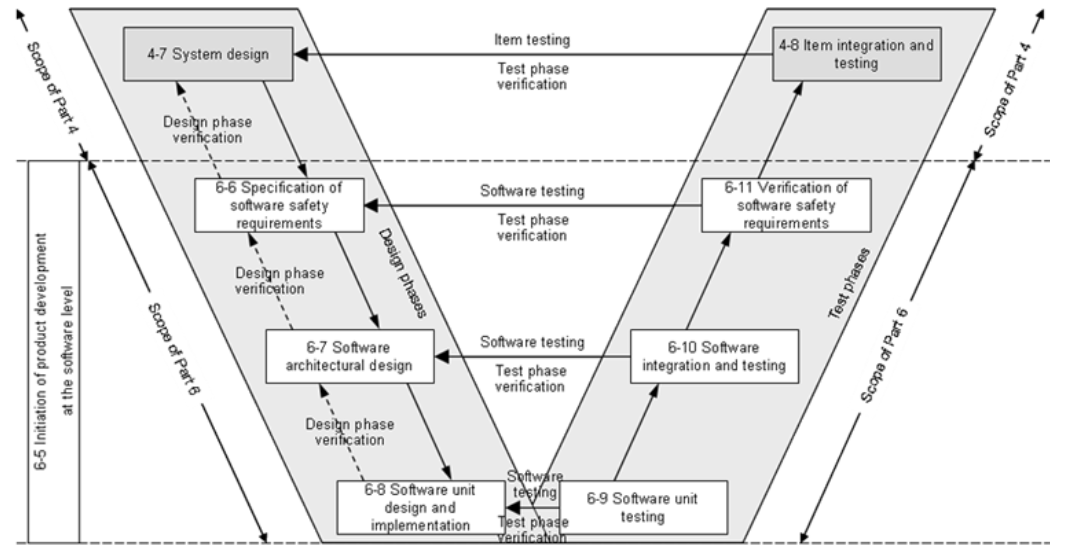
\includegraphics[keepaspectratio, width=\linewidth]{pictures/V}
  \label{IMG:phase_model}
  \caption{Phase model for software development}
\end{figure}

The first step is the system design. At this point the system specification is
written and then the software specifications. When all
specifications exists, the next phase is to design the software architecture.
The last part of the design is software unit design and implementation. All
phases must be a verification of the former phase.

When the implementation is done, it is time for the test phases. These begins
with software unit testing which tests the software unit design phase. If the
tests verifies that the software unit design and implementation is correct, the
test phase moves on to the architectural design and then to verification of
software safety requirements.
The last test phase verifies that the system is
designed according to the specification. %It is important that the test phases test the
% specifications and not the implementation.

\subsection{QuickCheck}
QuickCheck tests a program with a specification implemented as properties that
the program must hold \cite{QUICKCHECK:manual}. QuickCheck creates an arbitrary
test vector for each of the properties. Because it is arbitrary it can't be used
for true formal verification(?).

\subsection{Industrial standards}
Automotive software for safety related systems is required to be designed,
implemented and verified by the standard ISO~26262 that handles functional
safety for automotive equipment.
For a higher level of integrity ISO~26262 strongly recommends that a semi-formal
verification of each module should exist \cite[Table 9, part 6, p. 26]{ISO26262}.
It also recommends a formal verification, but because of the state-space
complexity this is hard to achieve.

ISO~26262 is built on IEC~61508 which is titled Functional Safety of
Electrical/Electro-nic/Programmable Electronic Safety-related Systems which can
be applied to any kind of industry. IEC~61508 have four safety integrity levels
(SIL) ranked 1-4. SIL 4 is the highest and sould be applied where a failure can
do devastating damage to a large area. The automotive industry is improbable to
have this risk. That is why ISO~26262 exists, it also has four levels of SIL
called automotive safety integrity level (ASIL). The ASIL range from A-D, where
D is the highest and roughly translated to SIL 3.

Some of the specifications in AUTOSAR is left quite open for interpretation.
This makes it possible for vehicle developers to have different specifications
for a configuration. Some parts of those configuration specifications is
generated into code, while other is manually written or added as configurables.

\subsection{Why Erlang?}
First of all Erlang can easily communicate with other programming language by
using byte streams. There have already been some work done including Erlang
AUTOSAR and QuickCheck, mostly by the QuviQ company\cite{QUVIQ:flyer}.
Imperative coding requires state based testing(?). There are a library in
Erlang developed by QuviQ for this purpose(?).

%Aim for the work. What should be accomplished?
\section{Purpose}
The purpose is to automate the testing process in an effective and good way
preferably using QuickCheck. To make it possible to raise the Automotive Safety
Integration Level (ASIL), in the software unit design and implementation phase
and in the software architectural design phase, a check must be done to see if
it exist a tool that can be used in order to perform a semi formal verification
of a module, and then make this process generalized for modules in
coexistence.\\

The purpose is also to be able to decrease the number of needed unit tests in
the software unit design and implementation phase. Even further is the goal to
introduce semi formal verification of the software architectural design face.

%question formulation?
%The problem at hand, the assignment
\section{Objective}
Propose and motivate what should be done to be able to achieve a semi-formal
verification. This should include a confidence interval for how certain the
verification is.

Prove that it is possible to do a semi-formal verification for an AUTOSAR module
and its specification, preferably using QuickCheck. This should be generalized
so its possible to test other specifications and modules at a later moment.
Also it should not matter which configuration that is active, because the
specification holds for all configurations.

%Limitations. What should be left out and why?
\section{Scope}
We will use AUTOSAR 4.0 revision 3 for our thesis work.
Since AUTOSAR consists of around 80 specifications and other auxiliary
materials\cite{AUTOSAR:URL}, we will limit our scope to one or two
specifications. The main module of this thesis is the CryptoServiceManager. This
module provides cryptographic functionalities for synchronous and asynchronous
services. This module is chosen because it only got a few dependencies, is used to trace
development and production errors but also to incorporate cryptographic
libraries.

It is hard to test that a call to another module gives the right results,
that is why we have chosen a module with a small number of
dependencies.
The CryptoServiceManager should also have functionality which gives the same
results no matter which state it is in, such as hash
functions\cite{SPEC:AUTOSAR:CSM}.

\subsection{Work flow}

\begin{enumerate}

\item Construct a model for AUTOSAR in Erlang
\item Run Quickcheck for this model and compare the results with the output from
the c code.
\item Tweak the generators \label{generators}
  \begin{itemize}
    \item Which test cases are relevant
    \item Evaluate the results
    \begin{enumerate}
      \item What is the state space?
      \item Collapse irrelevant states
    \end{enumerate}
  \end{itemize}
\item Are the results good enough?
\item If not go the step \ref{generators}
\end{enumerate}

%Method of accomplishment. How should the work be carried out?
\chapter{Method}
\section{Specification}
Specifications for what each module should do in AUTOSAR is given in text form.
Hence one must first, before a module can be tested, implement the specification
for that module in code.
\section{Testing}
Properties for a module have to take the current state in consideration since
most functions written in an imperative language are not immutable. This gives
raise to the idea of an state machine based testing tool.
\begin{itemize}
\item Choose a specification which will be translated to QuickCheck properties
in parts.
\item With the use of statistics and confidence intervals, show that, with
enough tests the state-space will be exhausted.
\item Evaluate other semi-formal techniques and show that the results from them
shows that QuickCheck is reliable for verification.
\item Generalize the technique.
\end{itemize}

\section{Implementation}
A challenging step is the analysing part. If the testing tool returns zero
errors what does that say about the robustness of the input byte code? Passed
100 of 100 tests is just a statement and does not say anything more than that
some tests passed. Can tests be implemented in a clever way so that it is
possible to get some kind of confidence interval on the correctness of the code?
\begin{figure}[!ht]
% Graphic for TeX using PGF
% Title: /home/oskar/documents/box.dia
% Creator: Dia v0.97.2
% CreationDate: Sat Sep  7 19:28:43 2013
% For: oskar
% \usepackage{tikz}
% The following commands are not supported in PSTricks at present
% We define them conditionally, so when they are implemented,
% this pgf file will use them.
\ifx\du\undefined
  \newlength{\du}
\fi
\setlength{\du}{15\unitlength}
\begin{tikzpicture}
\pgftransformxscale{1.000000}
\pgftransformyscale{-1.000000}
\definecolor{dialinecolor}{rgb}{0.000000, 0.000000, 0.000000}
\pgfsetstrokecolor{dialinecolor}
\definecolor{dialinecolor}{rgb}{1.000000, 1.000000, 1.000000}
\pgfsetfillcolor{dialinecolor}
\definecolor{dialinecolor}{rgb}{1.000000, 1.000000, 1.000000}
\pgfsetfillcolor{dialinecolor}
\fill (6.000000\du,7.000000\du)--(6.000000\du,11.000000\du)--(10.795000\du,11.000000\du)--(10.795000\du,7.000000\du)--cycle;
\pgfsetlinewidth{0.100000\du}
\pgfsetdash{}{0pt}
\pgfsetdash{}{0pt}
\pgfsetmiterjoin
\definecolor{dialinecolor}{rgb}{0.000000, 0.000000, 0.000000}
\pgfsetstrokecolor{dialinecolor}
\draw (6.000000\du,7.000000\du)--(6.000000\du,11.000000\du)--(10.795000\du,11.000000\du)--(10.795000\du,7.000000\du)--cycle;
% setfont left to latex
\definecolor{dialinecolor}{rgb}{0.000000, 0.000000, 0.000000}
\pgfsetstrokecolor{dialinecolor}
\node at (8.397500\du,9.195000\du){Testing Tool};
\pgfsetlinewidth{0.100000\du}
\pgfsetdash{}{0pt}
\pgfsetdash{}{0pt}
\pgfsetbuttcap
{
\definecolor{dialinecolor}{rgb}{0.000000, 0.000000, 0.000000}
\pgfsetfillcolor{dialinecolor}
% was here!!!
\pgfsetarrowsend{stealth}
\definecolor{dialinecolor}{rgb}{0.000000, 0.000000, 0.000000}
\pgfsetstrokecolor{dialinecolor}
\draw (10.795000\du,9.000000\du)--(12.000000\du,9.050000\du);
}
\pgfsetlinewidth{0.100000\du}
\pgfsetdash{}{0pt}
\pgfsetdash{}{0pt}
\pgfsetbuttcap
{
\definecolor{dialinecolor}{rgb}{0.000000, 0.000000, 0.000000}
\pgfsetfillcolor{dialinecolor}
% was here!!!
\pgfsetarrowsend{stealth}
\definecolor{dialinecolor}{rgb}{0.000000, 0.000000, 0.000000}
\pgfsetstrokecolor{dialinecolor}
\draw (0.000000\du,9.000000\du)--(6.000000\du,9.000000\du);
}
% setfont left to latex
\definecolor{dialinecolor}{rgb}{0.000000, 0.000000, 0.000000}
\pgfsetstrokecolor{dialinecolor}
\node[anchor=west] at (8.397500\du,9.000000\du){};
% setfont left to latex
\definecolor{dialinecolor}{rgb}{0.000000, 0.000000, 0.000000}
\pgfsetstrokecolor{dialinecolor}
\node[anchor=west] at (0.000000\du,10.000000\du){Module byte code};
% setfont left to latex
\definecolor{dialinecolor}{rgb}{0.000000, 0.000000, 0.000000}
\pgfsetstrokecolor{dialinecolor}
\node[anchor=west] at (3.000000\du,8.000000\du){};
% setfont left to latex
\definecolor{dialinecolor}{rgb}{0.000000, 0.000000, 0.000000}
\pgfsetstrokecolor{dialinecolor}
\node[anchor=west] at (2.000000\du,5.000000\du){Module specfication};
\definecolor{dialinecolor}{rgb}{1.000000, 1.000000, 1.000000}
\pgfsetfillcolor{dialinecolor}
\fill (12.000000\du,7.000000\du)--(12.000000\du,11.100000\du)--(17.800000\du,11.100000\du)--(17.800000\du,7.000000\du)--cycle;
\pgfsetlinewidth{0.100000\du}
\pgfsetdash{}{0pt}
\pgfsetdash{}{0pt}
\pgfsetmiterjoin
\definecolor{dialinecolor}{rgb}{0.000000, 0.000000, 0.000000}
\pgfsetstrokecolor{dialinecolor}
\draw (12.000000\du,7.000000\du)--(12.000000\du,11.100000\du)--(17.800000\du,11.100000\du)--(17.800000\du,7.000000\du)--cycle;
% setfont left to latex
\definecolor{dialinecolor}{rgb}{0.000000, 0.000000, 0.000000}
\pgfsetstrokecolor{dialinecolor}
\node at (14.900000\du,9.245000\du){};
\pgfsetlinewidth{0.100000\du}
\pgfsetdash{}{0pt}
\pgfsetdash{}{0pt}
\pgfsetmiterjoin
\pgfsetbuttcap
{
\definecolor{dialinecolor}{rgb}{0.000000, 0.000000, 0.000000}
\pgfsetfillcolor{dialinecolor}
% was here!!!
\pgfsetarrowsend{stealth}
{\pgfsetcornersarced{\pgfpoint{0.000000\du}{0.000000\du}}\definecolor{dialinecolor}{rgb}{0.000000, 0.000000, 0.000000}
\pgfsetstrokecolor{dialinecolor}
\draw (1.000000\du,5.000000\du)--(1.000000\du,6.000000\du)--(8.000000\du,6.000000\du)--(8.000000\du,7.000000\du);
}}
% setfont left to latex
\definecolor{dialinecolor}{rgb}{0.000000, 0.000000, 0.000000}
\pgfsetstrokecolor{dialinecolor}
\node at (14.900000\du,9.050000\du){Output};
% setfont left to latex
\definecolor{dialinecolor}{rgb}{0.000000, 0.000000, 0.000000}
\pgfsetstrokecolor{dialinecolor}
\node at (14.900000\du,9.850000\du){ analysis };
\end{tikzpicture}

\caption{Abstract implementation module}
\end{figure}

%Gantt-schema.
\chapter{Time-plan}
\section{Provisional plan}
Exactly how things should be done isn't clear. Therefor we are proposing a more
orderly plan to be able learn what can be done and where problems may lie a
head. At first just try to implement one or two simple rules from an AUTOSAR
specification, in Erlang, and try to run it on AUTOSAR module. It's important to
notice that this may have nothing to do with our final solution and is mostly
for evaluating what can be done in QuickCheck. Since our work is not just about
implementing tests, but rather show that we can make semi formal verification on
a module in AUTOSAR, the number of rules that we implement seems less relevant
than what we can do with the rules that we implement.

The next step is to analyse the results and come to a conclusion for how to
continue. Possible Erlang and QuickCheck is not suited for our goals.
More information about this can be found on the Gantt scheme
represented below.

\begin{ganttchart}[vgrid={dotted}, today=8, today label={Current week}, today offset=.5]{1}{20}
  \setganttlinklabel{s-s}{}
  \setganttlinklabel{f-s}{}
  \gantttitle{2013}{17}\gantttitle{2014}{3} \\
  \gantttitlelist{36,...,52,1,2,3}{1} \\
  %\ganttgroup{Group 1}{1}{10} \\
  \ganttbar[name=planning]{Planning}{1}{2} \\
  \ganttbar[name=research]{Research}{2}{5}\\
  \ganttbar[name=semiformal]{Semi formal verification}{2}{5}\\
  \ganttgroup[inline, group top shift=1.1, group left shift=0.4, group label font=\normalsize, group height=0.1]{Course}{2}{6}\\
  \ganttbar[name=course]{QuviQ Erlang course}{5}{5}\\
  \ganttbar[name=firsttest]{First test}{5}{5}\\
  \ganttbar[name=analysis]{Analysis of other tools}{2}{3}\ganttbar[name=analysis2]{}{5}{5}\\
  \ganttbar[name=decision]{Decision of technique}{6}{6} \\
  \ganttbar[name=implementation]{Implementation}{7}{10} \\
  \ganttbar[name=evaluation]{Evaluation of results}{11}{12}\\
  \ganttbar[name=focus]{Focus on thesis}{13}{15}\\
  \ganttmilestone[name=mecel]{Presentation to Mecel}{16}\\
  \ganttbar[name=polish]{Polish}{17}{20}\\
  \ganttbar[name=opposition]{Opposition}{17}{20}\\
  \ganttmilestone[name=chalmers]{Presentation to Chalmers}{20}\\
  \ganttbar{Thesis}{1}{20}
  \ganttlink{semiformal}{course} % semi formal - erlang course
  \ganttlink[link type=s-s]{course}{firsttest} % erlang course - first test
  \ganttlink[link type=f-s]{analysis}{firsttest} % other tools - first test
  \ganttlink[link type=f-s]{firsttest}{analysis2} % first test - other tools (end)
  \ganttlink[link type=f-s]{analysis2}{decision} % other tools - decision
  \ganttlink[link type=f-s]{decision}{implementation} % decision - implementation
  \ganttlink[link type=f-s]{implementation}{evaluation} % implementation - evaluation
%  \ganttlink[link type=f-s]{evaluation}{focus} % evaluation - focus on thesis
  \ganttlink{focus}{mecel} % focus on thesis - presentation to mecel
\end{ganttchart}

Finding out the exact definition of semi formal verification and getting an idea of how this
can be implemented is a fundamental step. Hence this is added explicitly, as
shown in the Gantt Scheme, to the project plan.
In the first test week we translate some specification
demands to QuickCheck code, and test if it is possible to prove that this is
semi formal verfied. The purpose of doing analysis of other tools is to see if there exists better
tools for our goals, we should then decide which tools and techniques to use.
A presentation to Mecel is planned to the last week in December.  In January we
present our work to Chalmers.


\bibliographystyle{vancouver}
\bibliography{references}


\end{document}
